% !TeX encoding = UTF-8
% !TeX spellcheck = en_US

\section{Evaluation and Future Work}
	\begin{frame}
		\frametitle{Contents}
		\tableofcontents[currentsection]
	\end{frame}
	\begin{frame}
		\frametitle{Evaluation and Future Work}
		\framesubtitle{Compliance with Requirements, JUnit Tests}
		\begin{itemize}
			\item Requirements fulfilled
				\begin{itemize}
					\item Application conditions only in DNF
					\item Limited set of attribute assignments and conditions
				\end{itemize}

			\only<2-3>{
			\item 2 JUnit test suites for 13 APIs with 90 test cases
				\begin{itemize}
					\item TestsuiteGT covers 90\,\% of the abstract classes and the interpreter
					\item Build of GT projects covers 94\,\% of the GT builder
					\item used in MBSE lecture (Summer Term 2018)
				\end{itemize}
			\item JUnit test suite for scoping/validation in the editor: 111 test cases, coverage 96\,\%
			}
		\end{itemize}
	\end{frame}
	\begin{frame}
		\frametitle{Evaluation and Future Work}
		\framesubtitle{End-User Survey: Textual Syntax and Visualization}
		\begin{center}
			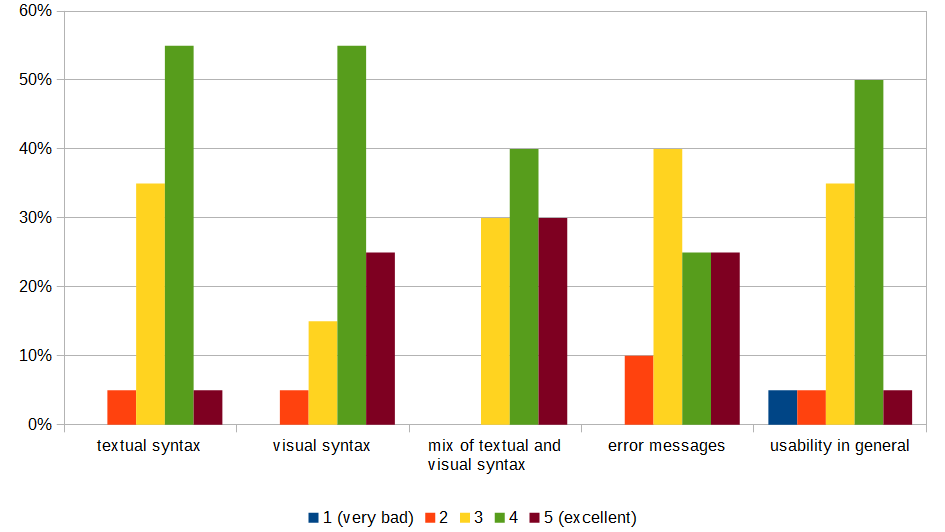
\includegraphics[width=\linewidth]{../common/figures/evaluation-results-syntax}
		\end{center}
	\end{frame}
	\begin{frame}
		\frametitle{Evaluation and Future Work}
		\framesubtitle{End-User Survey: Java Integration}
		\begin{center}
			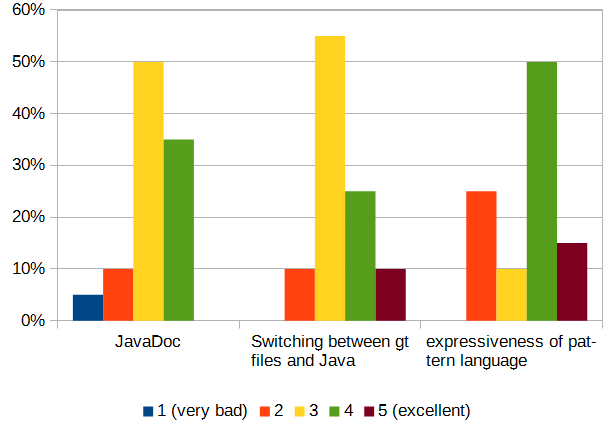
\includegraphics[width=.7\linewidth]{../common/figures/evaluation-results-java-integration}
		\end{center}
	\end{frame}
	\begin{frame}
		\frametitle{Evaluation and Future Work}
		\framesubtitle{Performance of Model Generation and Modification (linear time axis)}
		\begin{center}
			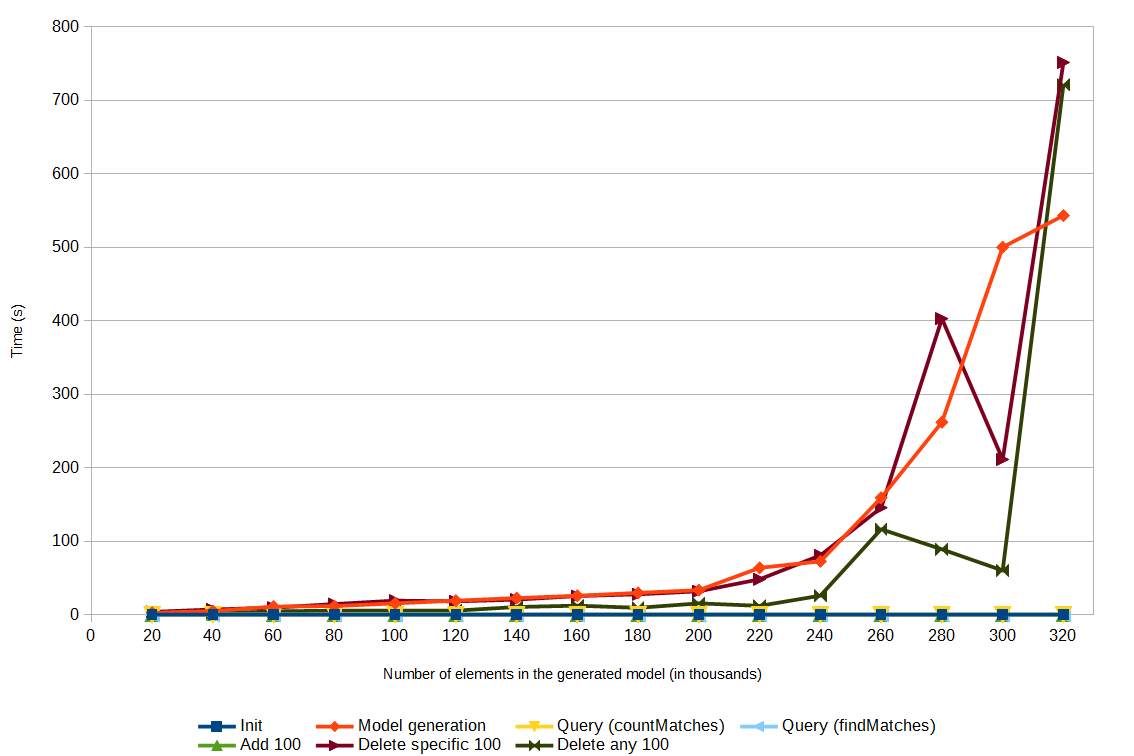
\includegraphics[height=.75\textheight]{../common/figures/evaluation-runtime1}
		\end{center}
	\end{frame}
	\begin{frame}
		\frametitle{Evaluation and Future Work}
		\framesubtitle{Performance of Model Generation and Modification (logarithmic time axis)}
		\begin{center}
			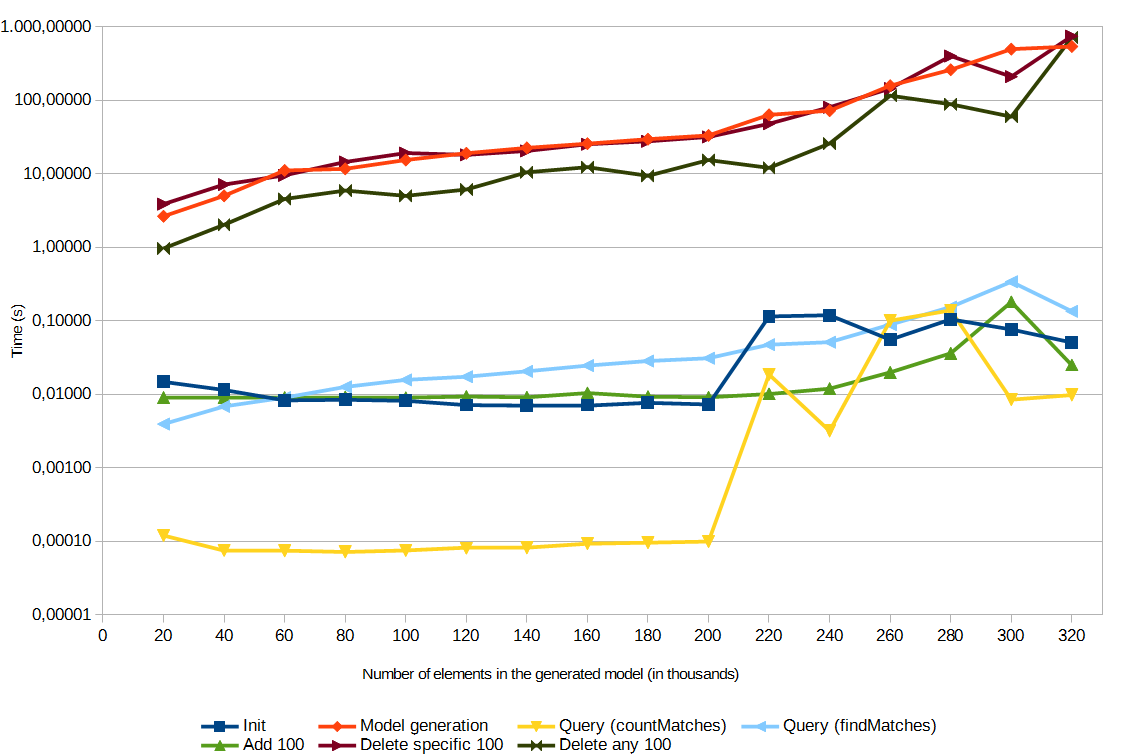
\includegraphics[height=.75\textheight]{../common/figures/evaluation-runtime1-logarithmic}
		\end{center}
	\end{frame}
	\begin{frame}
		\frametitle{Evaluation and Future Work}
		\framesubtitle{Performance of Model Queries (linear time axis)}
		\begin{center}
			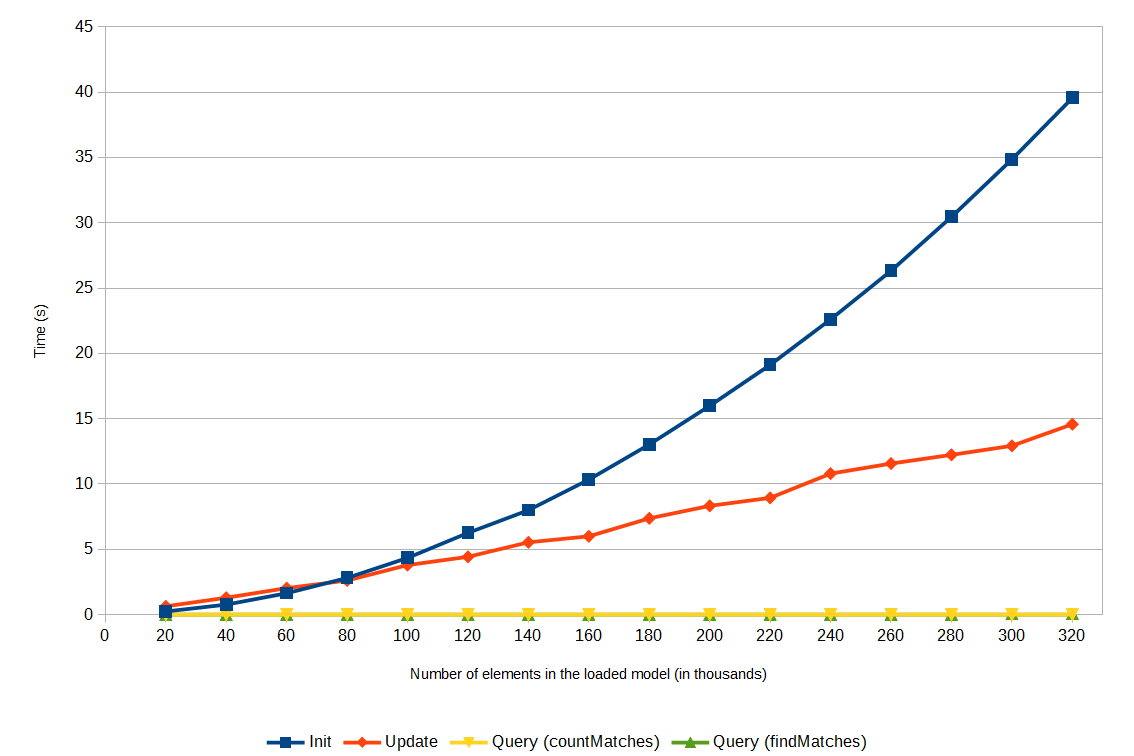
\includegraphics[height=.75\textheight]{../common/figures/evaluation-runtime2}
		\end{center}
	\end{frame}
	\begin{frame}
		\frametitle{Evaluation and Future Work}
		\framesubtitle{Performance of Model Queries (logarithmic time axis)}
		\begin{center}
			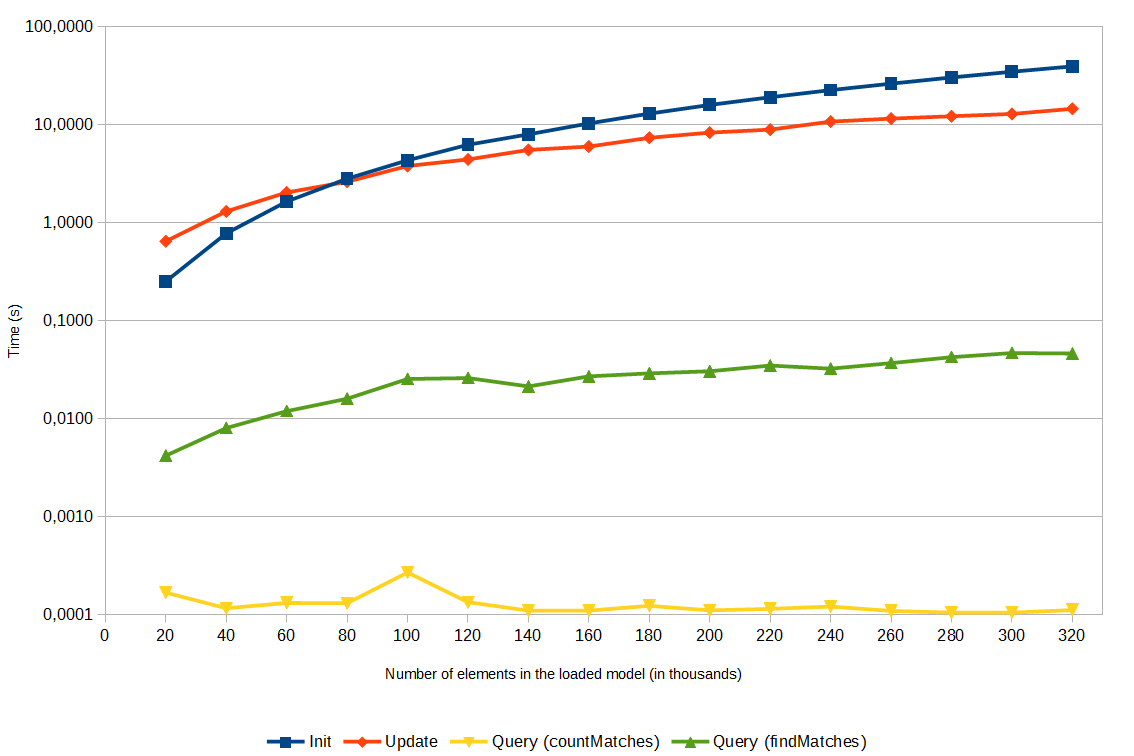
\includegraphics[height=.75\textheight]{../common/figures/evaluation-runtime2-logarithmic}
		\end{center}
	\end{frame}
	\begin{frame}
		\frametitle{Evaluation and Future Work}
		\framesubtitle{Summary and Future Work}
		\begin{block}{eMoflon::IBeX-GT}
			\begin{itemize}
				\item Expressive pattern language with simple syntax
				\item Integration into Java via a generated, typed API
				\item Incremental features
				\item Shared libraries with eMoflon::IBeX-TGG
			\end{itemize}
		\end{block}

		\only<2>{
		\begin{block}{Future work}
			\begin{itemize}
				\item Evaluation of performance
				\item Optimization of the pattern network
				\item Shared IBeX patterns with TGG
			\end{itemize}
		\end{block}
		}
	\end{frame}
